\subsection{Trace analysis}
\label{sec3.1-0}

In this chapter, we mainly introduce some phenomena and understandings observed through trace analysis. Since the average write traffic of the cluster in trace is much higher than the read traffic, we believe that the write traffic in the cloud environment is a more scarce resource. Therefore, the following paper explores the load balancing problem centering on the write traffic.

\subsubsection{Unbalanced network traffic distribution} 
\label{sec3.1-1}
\begin{table}[ht]
    %\footnotesize
    \small
    \centering
    \begin{tabular}{c|c|c}
         Cluster &Block server&Write traffic\\
         AY306L & 48 & 1.03E+13 \\
         AY251Z & 96 & 1.99E+13 \\
         AY272T & 82 & 2.35E+13 \\
         AY306O & 95 & 1.90E+13 \\
         AY336D & 96 & 2.05E+13 \\
         AY272M & 95 & 1.99E+13 \\
    \end{tabular}
    \caption{Cumulative write traffic}
    \label{table3.1-1}
\end{table}
\begin{figure}[ht]
    \centering
    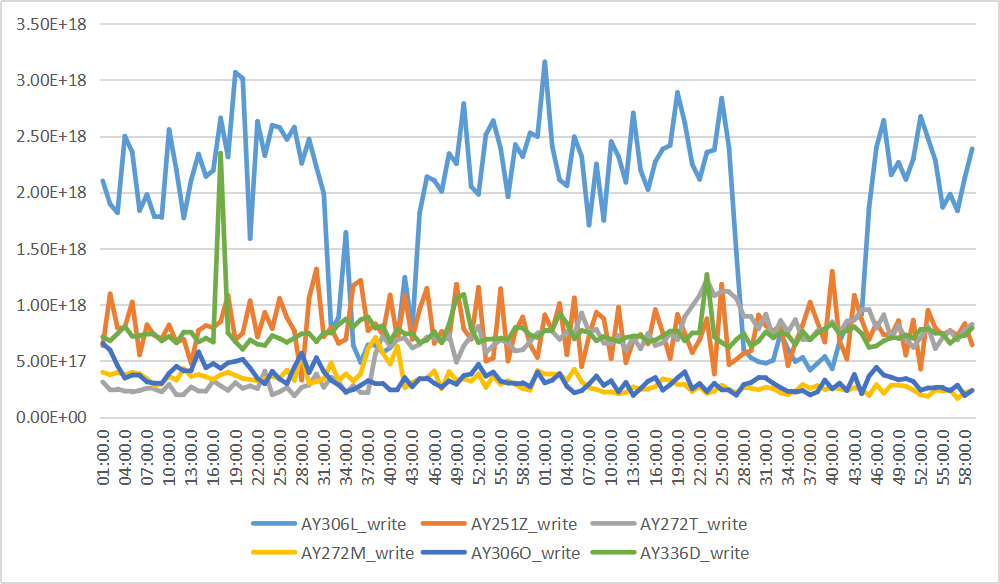
\includegraphics[width=0.4\textwidth]{Figure-3.1/Figure_3-1.png}
    \caption{Unbalance in different clusters}
    \label{fig3-1}
\end{figure}
We made a statistical analysis on the access and load balancing of the six clusters. First, we counted the cumulative write traffic of the six clusters in trace for two hours(Table \ref{table3.1-1}). We then calculated the variance of write traffic of different block servers in each cluster(Figure \ref{fig3-1}).Tthe vertical axis is the traffic variance of block server in the cluster, and the horizontal axis is the time, a serious imbalance can be obeserved.



\subsubsection{Impact of Group User}
\label{sec3.1-2}
First, we counted the cumulative traffic distribution in the segment. We observed that cloud disk of the same user may be similar in the write traffic characteristics. When the user scale is large and cloud disk has a large write traffic, it may have a great impact on the overall balance degree of the cluster. This kind of phenomenon appear in cluster AY272T and AY336D, their segment accumulated traffic and block server cumulative traffic as shown in figure,we can observe the four highest traffic segment belong to the same cloud disk, and their write traffic is very high, the cloud disk flow curve as shown in figure,It can be found that it is similar to the cluster balance degree curve characteristics, so it can be inferred that the balance degree fluctuation of cluster AY306L is affected by the cloud disk.


\subsubsection{Write Traffic Distribution of Segments}
\label{sec3.1-3}
First we delete cluster AY272T, AY336D from Figure \ref{fig3-1} to eliminate impact of group user.The write traffic variance of ESSD in the figure is greater than that of efficient disk. Based on this observation, we guess the cluster's traffic balance degree may be associated with the cloud disk performance, namely the high performance disk is more likely to cause imbalance phenomenon.

We observed the changes of block server traffic in different clusters and found that most of the write traffic fluctuations of block servers are not very large, but there are significant differences among different block servers(Figure \ref{fig3-2}).Occasionally there is a large fluctuation, but it is affected by  few segments of very high write traffic disk.Therefore, we assume that the segment traffic distribution is unbalanced, and this imbalance leads to traffic differences between block servers.To confirm our hypothesis,we calculated the cumulative write traffic of all segments(Figure \ref{fig3-3}), which is like the zipF distribution.Basically The top 10\% segments add up to 80\% of the total traffic.


Since the traffic difference between different segments may be large, the cluster balance degree is mainly affected by a small part of segments with higher traffic ranking.In order to observe the proportion and distribution of these segments in different clusters, we intercepted the segments whose cumulative traffic was greater than 1/10 of the average traffic of block servers for observation(Figure \ref{fig3-4}).
\begin{figure}[ht]
    \centering
    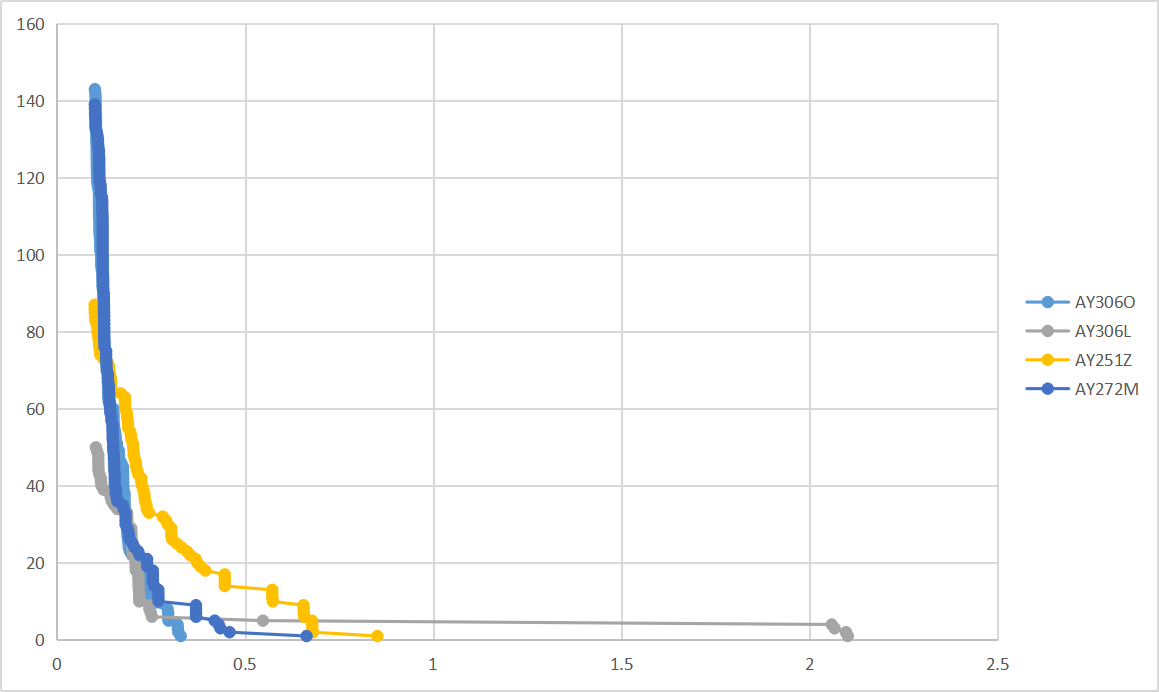
\includegraphics[width=0.4\textwidth]{Figure-3.1/Figure_3-3.png}
    \caption{Segment traffic distribution of different clusters}
    \label{fig3-4}
\end{figure}
(Figure \ref{fig3-4}).
It can be found that the curve of the high-performance disk approaches 0 at a slower speed, which indicates Among the few segments with the highest network traffic 
1. High performance clusters have higher peaks
2. High performance clusters Large degree of dispersion
As a result, the placement of these segments is more likely to cause imbalance